
\scsection{Введение в Технологию OSTIS}
\label{intro_ostis}

\begin{SCn}

\scnsectionheader{\currentname}

\scnstartsubstruct

\scnheader{Технология OSTIS}
\scnidtf{OSTIS}
\scnidtf{\uline{Открытая технология} проектирования \uline{совместимых} интеллектуальных систем}
\filemodetrue
\scnrelfromvector{предпосылки создания}{решение любой актуальной сложной (комплексной) задачи (понимание изображений, понимание текстов и речи, управление предприятиями и т.д.) требует комбинации в рамках системы различных \uline{видов знаний} (не только фактов, но и логических утверждений, ситуаций, событий, алгоритмов, т.д.) и различных \uline{моделей решения задач} (нейросетевых, логических, статистических моделей, классических алгоритмов и т.д.). При этом заранее нельзя сказать, какой именно набор понадобится для решения конкретной задачи.;
в настоящее время существуют системы, которые частично решают задачу интеграции различных моделей, однако такие системы делаются \uline{монолитными} и проектируются под \uline{конкретную задачу}. Разработка таких систем стоит огромных ресурсов, при этом развивать такие системы для решения других задач практически не представляется возможным, приходится делать все заново.}
\filemodefalse
\scnaddlevel{1}
\scnnote{В контексте \textit{Технологии OSTIS} мы считаем, что \uline{интеллектуальной} является не та система, которая может решить конкретную задачу (даже интеллектуальную), а та система, которая может легко \uline{обучаться} решению новых задач без существенных затрат.}
\scnaddlevel{-1}
\filemodetrue
\scnrelfromvector{принципы, лежащие в основе}{В основе \textit{Технологии OSTIS} лежит универсальный способ представления информации, названный \textit{SС-кодом}. В основу \textit{SC-кода} положены основные формализмы дискретной математики (теория множеств и теория графов), что обеспечивает как универсальность и унифицированность представления (можно представить любую информацию одинаковым образом), так и удобство обработки и восприятия человеком.;
Базовый \textit{Алфавит SC-кода} состоит всего из 5 элементов, на основе которых строятся все более сложные конструкции. При этом с помощью \textit{SC-кода} описываются не только знания системы, но и модели решения задач и даже интерфейс системы. Можно провести аналогию с тем, как из базового ограниченного набора элементарных частиц строятся различные вещества и далее различные объекты любой сложности.; 
Системы, построенные на основе \textit{Технологии OSTIS} (ostis-системы) состоят из \textit{базы знаний}, \textit{решателя задач} и \textit{интерфейса} взаимодействия с внешним миром (не обязательно пользовательского).;
\textit{База знаний ostis-системы} может описывать любые виды знаний, при этом легко дополняться новыми знаниями и новыми видами знаний.;
\textit{Решатель задач ostis-системы} основан на многоагентном подходе и позволяет легко интегрировать и комбинировать любые модели решения задач.;
\textit{Интерфейс ostis-системы} представляет собой совокупность специального вида \textit{базы знаний} и \textit{решателя задач}, т.е. также описывается средствами SC-кода.
}
\scnrelfromvector{преимущества}{В \uline{любую} ostis-систему без каких-либо \uline{накладных расходов} можно бесшовно \uline{интегрировать} любые \uline{знания} и \uline{модели решения задач} (по принципу plug\&play). Таким образом, не важно, что система умеет в данный момент, ее всегда можно переобучить на решение другой задачи.;
Разрабатываемые \uline{компоненты} ostis-систем \uline{универсальны} (могут использоваться в совершенно разных системах) и \uline{совместимы} между собой. Это означает, что можно накапливать \uline{библиотеку компонентов} и \uline{использовать компоненты повторно}, таким образом, сильно \uline{сокращается время разработки} каждой следующей системы. Например, в настоящее время универсальная часть (ядро) баз знаний позволяет сократить сроки разработки базы знаний новых систем на 40-60\%.;
За счет того, что вся система описывается средствами SC-кода, она может анализировать сама себя, искать в себе ошибки, оптимизировать собственную работу (обладает рефлексивностью). Рефлексивность считается одним из ключевых признаков интеллекта, даже люди далеко не всегда обладают рефлексивностью.;
За счет наличия базового \textit{Алфавита SC-кода} и возможности полного описания \textit{компьютерной системы} средствами \textit{SC-кода} возникает возможность сделать \textit{ostis-системы} полностью платформенно-независимыми (разделить модель системы и платформу интерпретации таких моделей). То есть разработка ostis-системы сводится к разработке ее модели и выполняется независимо не только от операционной системы, но и в принципе от архитектуры компьютера, на котором система работает. Платформа в свою очередь может быть реализована как \uline{программно} (наподобие виртуальной машины), так и \uline{аппаратно}.;
Как следует из предыдущего пункта, \textit{Технология OSTIS} является основной для нового типа компьютеров -- \uline{\textit{семантических компьютеров}}. В отличие от других компьютеров с нетрадиционной архитектурой (в том числе суперкомпьютеров), для которых не всегда понятно, как именно их использовать, для семантических компьютеров уже готова технология и конкретные системы, которые будут на них работать.;
За счет используемого в \textit{Технологии OSTIS} подхода к обработке информации (особого рода многоагентного подхода) ostis-системы оказываются изначально ориентированы на \uline{параллельную обработку информации}, в том числе, поддержку ее на аппаратном уровне (в рамках семантического компьютера).}
\filemodefalse
\scnaddlevel{1}
    \scntext{вывод}{Таким образом, по сравнению с традиционными технологиями, \textit{Технология OSTIS} позволяет при той же скорости обучения разработчиков и трудоемкости разработки новых компонентов значительно снизить сроки разработки систем за счет повторного использования компонентов и легкости их интеграции. При этом производительность \textit{ostis-системы} по сравнению с аналогичной традиционной системой в общем случае может оказаться ниже, но данная проблема будет решена при переходе на семантические компьютеры.

    При необходимости, \textit{ostis-система} может включать не только компоненты, разработанные на основе \textit{Технологии OSTIS}, но и легко интегрироваться с любыми другими системами и интегрировать другие компоненты посредством специального протокола обмена информацией и/или программного интерфейса (API). Такие компоненты не будут в полной мере обладать некоторыми важными свойствами ostis-систем (например, рефлексивностью) но это позволит заимствовать современные разработки и решить проблему производительности при решении наиболее ресурсоемких задач (например, при обучении нейросетей).
    }
\scnaddlevel{-1}
\scnnote{Важно отметить, что \uline{\textit{OSTIS} -- не конкретная интеллектуальная система} или способ решения задач какого-либо класса, это \uline{технология разработки интеллектуальных систем}, каждая из которых в свою очередь в каждый конкретный момент будет решать задачи определенного класса. При этом ключевые преимущества \textit{OSTIS} заключаются не в принципиально новых функциональных возможностях разрабатываемых систем (большинство \textit{ostis-систем} могут быть реализованы современными традиционными средствами), а в том, насколько легко можно \uline{модифицировать и развивать} разрабатываемые системы, адаптировать их под новые задачи, а также в том, насколько эффективно можно \uline{накапливать и использовать полученные компоненты} при разработке новых систем, снижая при этом сроки и трудоемкость их разработки.
}
\filemodetrue
\scnrelfromvector{текущий состав}{программная реализация платформы (модели семантического компьютера), которая лежит в основе каждой ostis-системы. Может использоваться как при разработке web-приложений, так и настольных и мобильных приложений.;
постоянно пополняемая \textit{Библиотека компонентов баз знаний ostis-систем}, включая универсальное \textit{Ядро баз знаний ostis-систем}. В текущий момент наличие данной библиотеки позволяет сократить сроки разработки баз знаний на 40-60\%.;
постоянно пополняемая \textit{Библиотека компонентов решателей задач ostis-систем}, включая механизмы поиска информации и некоторые модели решения задач, среди которых выделяется соответствующее \textit{Ядро решателей задач ostis-систем}. В настоящее время на первых этапах разработки системы оказывается достаточным использовать только \textit{Ядро решателей задач ostis-систем} и не разрабатывать дополнительно никаких компонентов.;
комплекс \textit{Средств информационной поддержки разработчиков ostis-систем} (включая описание самих моделей, а также методики и руководства), оформленных в виде интеллектуальной \textit{Метасистемы IMS.ostis} (IMS) и доступный онлайн \url{https://ims.ostis.net.}}

\scnrelfromvector{текущее применение}{на основе \textit{Технологии OSTIS} силами студентов и аспирантов активно развивается большое число открытых прототипов обучающих и справочных систем, которые можно найти на \url{https://github.com/ostis-apps};
разработки на основе \textit{Технологии OSTIS} успешно внедрены на ОАО ``Савушкин продукт''  при разработке системы информационного обслуживания сотрудников и при разработке компонентов систем контроля качества продукции;
\textit{Технология OSTIS} позволит значительно более эффективно реализовать анализ естественного языка (включая речь), в том числе для чат-ботов, синхронного перевода и речевых ассистентов. В настоящее время выполняется ряд проектов по данной тематике.}
\filemodefalse
\scntext{планы развития}{Предполагается, что в ближайшем будущем \textit{Метасистема IMS.ostis} и другие \textit{ostis-системы} будут объединены в распределенную облачную \textit{ostis-систему}, названную \textit{Экосистемой OSTIS}. Общая архитектура экосистемы показана на рисунке \textit{Архитектура Экосистемы OSTIS}. При этом все \textit{ostis-системы} в составе \textit{Экосистемы OSTIS} будут в каждый момент времени совместимы между собой, при этом совместимость будет контролироваться автоматически. Любой желающий сможет внести свой вклад в развитие любой из ostis-систем в составе \textit{Экосистемы OSTIS}, в первую очередь -- \textit{Метасистемы IMS.ostis}, при этом вклад будет автоматически верифицироваться и оцениваться. В то же время, как видно из представленной архитектуры, владельцы \textit{ostis-систем} смогут самостоятельно выбирать, какой частью своей информации они готовы поделиться с другими пользователями \textit{Экосистемы OSTIS}, персональная же часть информации будет гарантированно защищена.}

\scnheader{Архитектура Экосистемы OSTIS}
\scneqimage{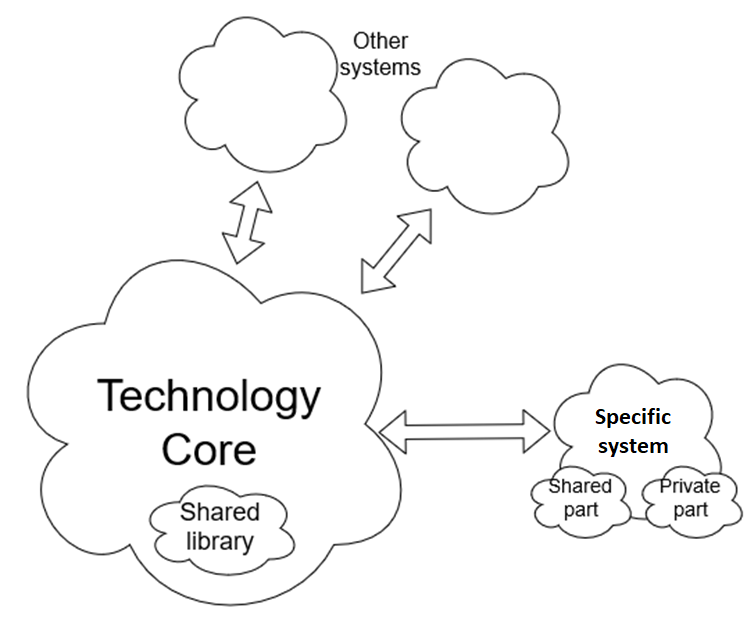
\includegraphics[width=0.6\textwidth]{figures/chapter0/ecosystem.png}}

\scnheader{Технология OSTIS}
\scnrelfromvector{текущие проекты}{Проект Экосистема OSTIS;Проект Метасистема IMS.ostis;Проект Семейство различных вариантов реализации универсального интерпретатора семантических моделей интеллектуальных систем\\
\scnaddlevel{1}
    \scnrelfromlist{подпроект}{Проект Программно реализованный на современных компьютерах универсальный интерпретатор семантических моделей интеллектуальных систем;Проект Семантический ассоциативный компьютер}
\scnaddlevel{-1}
;Проект Комплекс совместимых средств проектирования интеллектуальных систем\\
\scnaddlevel{1}
    \scnrelfromlist{подпроект}{Проект Встраиваемая типовая интеллектуальная система комплексной поддержки проектирования баз знаний;Проект Интеллектуальная система комплексной поддержки проектирования решателей задач интеллектуальных систем;Проект Интеллектуальная система комплексной поддержки проектирования вербальных интерфейсов интеллектуальных систем;Проект Интеллектуальная система комплексной поддержки проектирования невербальных интерфейсов}
\scnaddlevel{-1}
;Проект Семейство совместимых интеллектуальных справочных, обучающих и help-систем\\
\scnaddlevel{1}
    \scnrelfromlist{подпроект}{Проект Специализированные средства разработки совместимых интеллектуальных справочных, обучающих и help-систем различного назначения;Проект Комплекс семантически совместимых интеллектуальных справочных и обучающих систем по всем дисциплинам среднего образования;Проект Комплекс семантически совместимых интеллектуальных справочных и обучающих систем по всем дисциплинам, являющихся базовыми при подготовке инженеров по информационным специальностям;Проект Комплекс семантически совместимых интеллектуальных справочных и обучающих систем по всем специальным дисциплинам специальности ''Искусственный интеллект''{};Проект Семейство совместимых интеллектуальных справочных и обучающих систем по стандартам различного вида}
\scnaddlevel{-1}
;Проект Семейство совместимых интеллектуальных корпоративных систем ситуационного управления\\
\scnaddlevel{1}
    \scnrelfromlist{подпроект}{Проект Интеллектуальная корпоративная система ситуационного управления предприятием рецептурного производства;Проект Интеллектуальная корпоративная система ситуационного управления деятельностью выпускающей кафедры технического вуза}
\scnaddlevel{-1}
}
\scnrelfromvector{будущие проекты}{
Проект Семейство совместимых интеллектуальных систем автоматизации проектирования в различных областях;Проект Семейство совместимых порталов знаний\\
\scnaddlevel{1}
    \scnrelfrom{подпроект}{Проект Портал научных знаний по искусственному интеллекту}
\scnaddlevel{-1}
;Проект Семейство совместимых интеллектуальных систем экскурсионного обслуживания;Проект Семейство совместимых интеллектуальных геоинформационных систем;Проект Семейство совместимых интеллектуальных робототехнических систем и специализированных средств их разработки;Проект Семейство совместимых интеллектуальных систем персонального обслуживания и мониторинга\\
\scnaddlevel{1}
    \scnrelfromlist{подпроект}{Проект Интеллектуальная система персонального обслуживания и мониторинга пользователей и разработчиков компьютерных систем, входящих в Экосистему OSTIS;Проект Интеллектуальный персональный ассистент по взаимодействию с традиционными internet-системами и их пользователями;Проект Интеллектуальная система персонального комплексного медицинского мониторинга и контроля}
\scnaddlevel{-1}
}

\scnsegmentheader{Понятие технологии OSTIS}

\scnstartsubstruct

\scnheader{Технология OSTIS}
\scnidtf{Комплекс (семейство) технологий, обеспечивающих проектирование, производство, эксплуатацию и реинжиниринг интеллектуальных \textit{компьютерных систем (ostis-систем)}, предназначенных для автоматизации самых различных видов человеческой деятельности и в основе которых лежит смысловое представление и онтологическая систематизация знаний, а также агентно-ориентированная обработка знаний}
\scnidtf{Open Semantic Technology for Intelligent Systems}
\scnaddlevel{1}
\scntext{сокращение}{OSTIS}
\scnaddlevel{-1}
\scnidtf{Семейство (комплекс) \textit{ostis-технологий}}
\scnidtf{Комплексная открытая семантическая технология проектирования, производства, эксплуатации и реинжиниринга гибридных, семантически совместимых, активных и договороспособных \textit{интеллектуальных компьютерных систем}}
\scnheader{Технология OSTIS}
\scnrelfromset{принципы, лежащие в основе}{
\scnfileitem{Ориентация на разработку \textit{интеллектуальных компьютерных систем}, имеющих высокий уровень \textit{интеллекта} и, в частности, высокий уровень \textit{социализации}. Указанные системы, разработанные по \textit{Технологии OSTIS}, будем называть \textbf{ostis-системами}}
;\scnfileitem{Ориентация на \uline{комплексную} автоматизацию всех видов и областей \textit{человеческой деятельности} путем создания сети взаимодействующих и координирующих свою деятельность \textit{ostis-систем}. Указанную сеть \textit{ostis-систем} вместе с их пользователями будем называть \textbf{\textit{Экосистемой OSTIS}}}
;\scnfileitem{Поддержка перманентной эволюции \textit{ostis-систем} в ходе их эксплуатации.}
;\scnfileitem{\textit{Технология OSTIS} реализуется в виде сети \textit{ostis-систем}, которая является частью \textit{Экосистемы OSTIS}.
Ключевой \textit{ostis-системой} указанной сети является \textbf{Метасистема IMS.ostis} (Intelligent MetaSystem), реализующая \textbf{Ядро Технологии OSTIS}, которое включает в себя базовые (предметно независимые) методы и средства проектирования и производства \textit{ostis-систем} с интеграцией в их состав типовых встроенных подсистем поддержки эксплуатации и реинжиниринга \textit{ostis-систем}. Остальные \textit{ostis-системы}, входящие в состав рассматриваемой сети, реализуют различные специализированные \textit{ostis-технологии} проектирования различных классов \textit{ostis-систем}, обеспечивающих автоматизацию любых областей и \textit{видов человеческой деятельности}, кроме \textit{проектирования ostis-систем}.}
;\scnfileitem{Конвергенция и интеграция на основе смыслового представления знаний всевозможных научных направлений \textit{Искусственного интеллекта} (в частности, всевозможных базовых знаний и навыков решения интеллектуальных задач) в рамках \textit{Общей формальной семантической теории ostis-систем}.}
;\scnfileitem{Ориентация на разработку компьютеров нового поколения, обеспечивающих эффективную (в том числе, производительную) интерпретацию логико-семантических моделей \textit{ostis-систем}, представленных базами знаний этих систем и имеющих смысловое представление.}}

\scnsegmentheader{Понятие ostis-системы}

\scnstartsubstruct

\scnheader{ostis-система}
\scnidtf{\textit{интеллектуальная компьютерная система}, спроектированная и реализованная по требованиям и стандартам \textit{Технологии OSTIS}, которые задокументированы в \textit{Общей теории ostis-систем}}

\scnheader{ostis-система}
\scnidtf{интеллектуальная компьютерная система, построенная в соответствии с принципами и требованиями Технологии OSTIS}
\scnidtf{Множество ostis-систем различного назначения}
\scnaddlevel{1}
\scniselement{имя собственное}
\scnaddlevel{-1}
\scnidtf{Множество всевозможных интеллектуальных компьютерных систем, построенных по Технологии OSTIS}

\scnheader{ostis-система}
\scnsubset{интеллектуальная компьютерная система}
\scnidtf{\textit{интеллектуальная компьютерная система}, которая построена в соответствии с требованиями и стандартами \textit{Технологии OSTIS}, что обеспечивает существенное развитие целого ряда \textit{свойств} (способностей) этой \textit{компьютерной системы}, позволяющих значительно повысить \textit{уровень интеллекта} этой системы (и, прежде всего, ее \textit{уровень обучаемости} и \textit{уровень социализации})} 

\scnauthorcomment{Добавить классификацию из пояснения}

\scnsubdividing{индивидуальная ostis-система;коллективная ostis-система\\
\scnaddlevel{1}
    \scnsubdividing{простой коллектив ostis-систем;иерархический коллектив ostis-систем}   
\scnaddlevel{-1}
}

\scnheader{ostis-система}
\scnexplanation{интеллектуальная компьютерная система, разработанная, разрабатываемая или совершенствуемая по технологии OSTIS}
\scnnote{Когда речь идет о таком компоненте технологии OSTIS, как модели ostis-систем, фактически имеется в виду теория ostis-систем, включающая в себя строгое формальное уточнение того, как устроена ostis-система, какова ее архитектура, принципы организации памяти, принципы организации представления информации, принципы организации интерфейса с внешней средой (в том числе, с пользователями)}

\scnheader{ostis-система}
\scnrelfromset{принципы, лежащие в основе}{
\scnfileitem{Информация, хранимая в памяти \textit{ostis-системы}, имеет смысловое представление.}
;\scnfileitem{В основе организации решения задач в памяти \textit{ostis-системы} лежит \textit{агентно-ориентированная модель обработки информации}, управляемая ситуациями и событиями, возникающими в обрабатываемой информации (точнее, в обрабатываемой базе знаний).}
;\scnfileitem{Унификация базового набора (базовой системы) используемых понятий, что является основой обеспечения \textit{семантической совместимости} всех \textit{ostis-систем}.}
;\scnfileitem{В основе структуризации информации (базы знаний), хранимой в памяти \textit{ostis-системы}, лежит иерархическая система \textit{предметных областей} и соответствующих им \textit{формальных онтологий}.}
;\scnfileitem{Способность к пониманию (к семантическому погружению, к семантической интеграции) новых приобретаемых знаний (и, в том числе, новых навыков) в состав текущего состояния \textit{базы знаний}.}
;\scnfileitem{Способность к \textit{семантической конвергенции} (к обнаружению сходств) новых приобретаемых знаний (и, в частности, навыков) со знаниями, входящими в состав текущего состояния базы знаний \textit{ostis-системы}.}
;\scnfileitem{Способность \textit{ostis-системы} поддерживать высокий уровень своей \textit{семантической совместимости} (высокий уровень взаимопонимания) с другими \textit{ostis-системами}.}
;\scnfileitem{Способность ostis-системы согласовывать, координировать свою деятельность с другими \textit{ostis-системами}.}
;\scnfileitem{\scnauthorcomment{статья на OSTIS-2020}}
;\scnfileitem{\scnauthorcomment{статья на OSTIS-2020}}
;\scnfileitem{\scnauthorcomment{статья на OSTIS-2020}}
;\scnfileitem{\scnauthorcomment{статья на OSTIS-2020}}}
\scntext{следовательно}{Перечисленные свойства \textit{ostis-систем} свидетельствуют о том, что они имеют существенно более высокий \textit{уровень интеллекта} и, в частности, более высокий \textit{уровень социализации} по сравнению с современными \textit{интеллектуальными компьютерными системами}. \scnauthorcomment{См. начало Раздела 1.1}}

\scnheader{ostis-система}
\scnrelfromset{принципы, лежащие в основе}{
\scnfileitem{смысловое представление информации в памяти компьютерных систем, направленное на устранение недостатков современных компьютерных систем и технологий путем повышения уровня интеллектуальности компьютерных систем}
;\scnfileitem{децентрализация управления решателем задач
\begin{itemize}
	\item внутренняя МАС
	\item внешняя МАС
\end{itemize}}
;\scnfileitem{интеграция различных видов знаний}
;\scnfileitem{интеграция различных моделей решателей задач}
;\scnfileitem{ориентация на компьютеры нового поколения}
;\scnfileitem{обеспечение семантической совместимости компьютерных систем}
;\scnfileitem{обеспечение поддержания семантической совместимости компьютерных систем в ходе эволюции}
;\scnfileitem{способность к координации деятельности}}

\scnheader{ostis-система}
\scnrelfromset{принципы, лежащие в основе}{
\scnfileitem{Память ostis-системы является графодинамической (т.е. нелинейной (графовой) и структурно перестраиваемой). Переработка информации в памяти ostis-системы сводится не столько к изменению состояния элементов памяти (это происходит только при изменении синтаксического типа элементов и при изменении содержимого тех элементов, которые обозначают файлы), сколько к изменению \uline{конфигурации связей} между ними.}
;\scnfileitem{Хранение информации в памяти ostis-системы ориентируется на \uline{смысловое} представление информации – без синонимов, омонимов знаков и без семантической эквивалентности информационных конструкций.}
;\scnfileitem{С точки зрения архитектуры ostis-система представляет собой \uline{иерархическую} многоагентную систему с общедоступной памятью (т.е. с памятью, общедоступной \uline{всем} агентам ostis-системы). 
Заметим при этом, что общая память большинства исследуемых в настоящее время многоагентных систем является не общедоступной, а распределенной, т.е. представляет собой абстрактное (виртуальное) объединение, в состав которого входит память каждого агента многоагентной системы. Координация деятельности агентов ostis-системы при выполнении сложных \textit{действий в памяти} ostis-системы реализуется также через \textit{память ostis-системы} с помощью хранимых в памяти \textit{методов} решения различных классов задач, а также с помощью хранимых в памяти \textit{планов} решения конкретных задач.
На основании этого можно строить неограниченную иерархическую систему агентов ostis-системы – от элементарных агентов, обеспечивающих выполнение базовых действий в памяти ostis-системы, до неэлементарных агентов, представляющих собой коллективы (группы) элементарных и/или неэлементарных агентов, обеспечивающих решение различных типовых задач с помощью соответствующих методов и планов.}
;\scnfileitem{Организация выполнения \textit{ostis-системой действий во внешней среде} осуществляется следующим образом:
\begin{scnitemize}
	\item Выделяются классы \textit{элементарных действий во внешней среде}, для реализации каждого из которых вводятся \textit{эффекторные агенты} ostis-системы.
	\item Координация деятельности \textit{эффекторных агентов} ostis-системы при выполнении \textit{сложных действий во внешней среде} осуществляется через \textit{память ostis-системы} с помощью хранимых в памяти \textit{методов} и \textit{планов} решения различных задач во \textit{внешней среде}, а также с помощью \textit{рецепторных агентов} ostis-системы, обеспечивающих обратную связь и, соответственно, сенсомоторную координацию.
\end{scnitemize}}}

\scnheader{ostis-система}
\scnrelfromset{принципы, лежащие в основе}{
\scnfileitem{Способность понимать друг друга, а также любого своего пользователя
\scnaddlevel{-2}
\scnidtf {Совместимость используемых понятий (по терминам и по денотационной семантике)}
\scnidtf {Семантическая совместимость}
\scnaddlevel{2}}
;\scnfileitem{Способность поддерживать взаимопонимание в процессе индивидуальной эволюции, приводящей к расширению и/или корректировке системы используемых понятий}
;\scnfileitem{Способность координировать свою деятельность с другими системами при решении задач, которые усилиями одной (индивидуальной) интеллектуальной компьютерной системы не могут быть решены либо принципиально, либо за разумное время}}

\scnheader{ostis-система}
\scnrelfromset{принципы, лежащие в основе}{
\scnfileitem{Высокая степень индивидуальной обучаемости интеллектуальных компьютерных систем
\begin{itemize}
	\item гибкости
	\item стратифицированности
	\item рефлексивности
	\item универсальность средств представления и образования знаний
\end{itemize}}
;\scnfileitem{Высокая степень семантической совместимости и, как следствие, коллективной обучаемости интеллектуальных компьютерных систем
\begin{itemize}
	\item семантической совместимости
\end{itemize}}
;\scnfileitem{Основа для автоматизации рынка знаний}}

\scnmakeset{память*;ostis-система}
\scnrelfrom{сужение второго домена заданного отношения для заданного первого домена}{память ostis-системы}
\scnaddlevel{1}
\scnsubset{смысловая память}
\scnaddlevel{-1}


\scnmakeset{информация, хранимая в памяти кибернетической системы*;  ostis-система}
\scnrelfrom{сужение второго домена заданного отношения для заданного первого домена}{база знаний ostis-системы}
\scnaddlevel{1}
\scnsubset{смысловое представление информации}
\scnaddlevel{-1}


\scnheader{память ostis-системы}
\scnsubset{смысловая память}

\scnheader{информация, хранимая в памяти ostis-системы}
\scnsubset{смысловое представление информации}

\scnheader{решатель задач ostis-системы }
\scnsubset{агентно-ориентированная модель обработки информации в памяти}







































 

\scnendstruct

\end{SCn}
